%*******************************************************************************
%*********************************** Chapter XXXXXXXX *****************************
%*******************************************************************************

\chapter{Simulations of the DUNE Far Detector}  %Title of chapter
\graphicspath{{FarDetectorSimulations/Figs/Raster/}{FarDetectorSimulations/Figs/PDF/}{FarDetectorSimulations/Figs/}}

Previous work presented has been done concerning the 35 ton prototype, however it is also important to simulate the DUNE Far Detector (FD). Simulations in the FD have concentrated on cosmogenic background to neutrino oscillations, in Section~\ref{sec:LBNESurf}, and the muon background to nucleon decay, in Section~\ref{sec:DUNENDK}. The simulations shown in Section~\ref{sec:LBNESurf} are discussed in!!!!~citep{MartinsThesis}!!!!, and were performed for the Long Baseline Neutrino Experiment (LBNE), which along with the Long Baseline Neutrino Oscillation (LBNO) experiment formed the basis for DUNE, and so are included here for completeness. The other work presented was performed for the DUNE collaboration in conjunction with work done by Vitaly Kudryavtsev and Matthew Robinson, both of the University of Sheffield, and was performed with the aim of producing muon-induced background limits to nucleon decay. \\

%********************************** %Second Section  **************************************
\section{Simulations of the LBNE surface detector} \label{sec:LBNESurf} %Section - X.2

%********************************** % Third Section  *************************************
\section{The use of MUSUN in LArSoft} \label{sec:FDIncorporation}  %Section - X.3
The primary muons in the following discussions are all generated using MUSIC~\citep{MUSUN}~\citep{MUSIC}~\citep{MUSIC2} and MUSUN~\citep{MUSUN}~\citep{MUSUN2}, and so a brief overview of them is required. MUSIC first propagates muons through a medium, defined by the user, for given initial energies, positions, and direction cosines. A range of energies between 10$^2$ and 10$^7$ GeV are considered, and their energy distributions are stored at depths of between 100 and 15,000 m w.e. Energy losses due to four processes are considered; ionisation, bremsstrahlung, electron-positron pair production and muon-nucleus inelastic scattering. The output of MUSIC is then used by MUSUN to generate a muon energy spectrum and angular distribution, for a given detector location. MUSUN is able to use information about the local surface profile to make these distributions more accurate. \\

The location of the DUNE far detector, near the Ross shaft at SURF, has global coordinates of; latitude = 44$^{\circ|}$20$'$45.21$''$ North, longitude 103$^{\circ}$45$'$16.13$''$ West. The rock composition is assumed to be; $< Z >$ = 12.09, $< A >$ = 24.17. The density is assumed to be 2.70 g cm${-3}$~\citep{Mei:2009py}. The flux calculated by MUSIC/MUSUN of 5.18 $\times$ 10$^{-9}$ cm$^{-2}$ s$^{-1}$ sr$^{-1}$ is well matched to the flux measured by the active veto system of the Davis' experiment, which was (5.38 $\pm$ 0.07) $\times$ 10$^{-9}$ cm$^{-2}$ s$^{-1}$ sr$^{-1}$~\citep{PhysRevD.27.1444}. Given the small differences in these values, and another measurement by the Majorana demonstrator, the systematic uncertainty in calculating the muon flux is estimated to be 20\%~\citep{NDKTFNote}. \\

The surface profile around the proposed detector location is shown in Figure~\ref{fig:SurfProf_Col}, where the proposed location is in the centre of the map. Each quadrant on the map has been divided into 4 angles of 22$^{\circ}$ to help guide the eye when comparing to Figure~\ref{fig:SurfProf_Azi}, where the distribution of azimuth angles is plotted. The vertical lines in Figure~\ref{fig:SurfProf_Azi} show the division of the quadrants when the angle is calculated from East to the North. When moving from East to North it is possible to discern how the peaks and troughs on the surface profile, correspond to troughs and peaks, in the distribution of azimuthal angle. \\

\begin{figure}[h!]
  \centering
  \begin{subfigure}{0.45\textwidth}
    \centering
    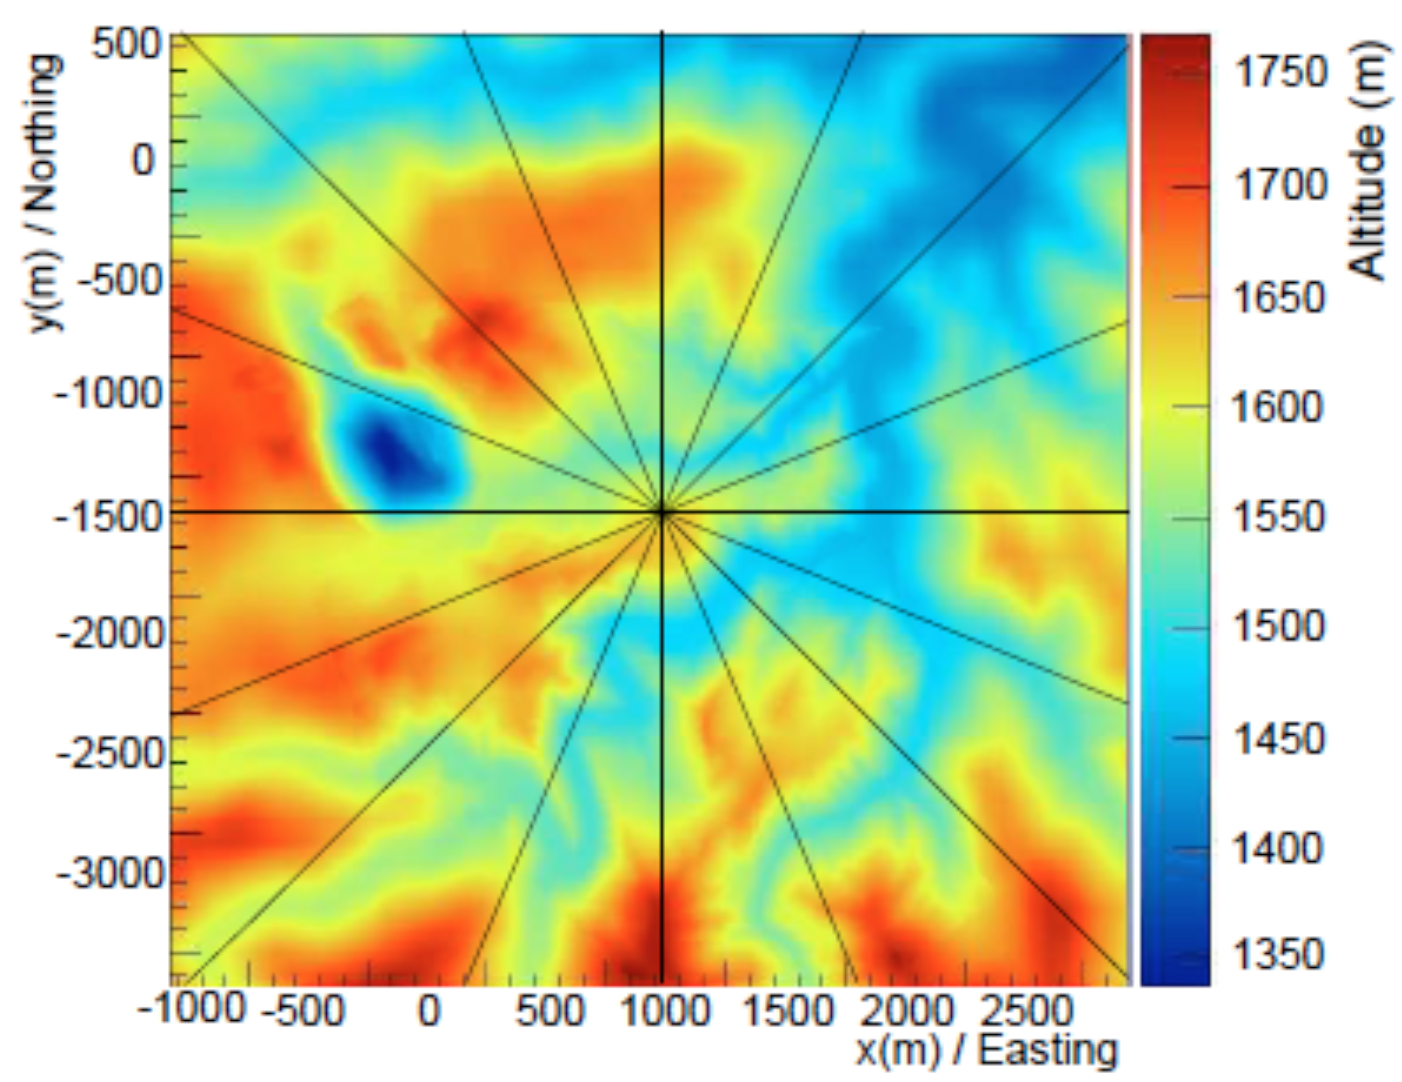
\includegraphics[width=\textwidth]{dune-surface-map}
    \caption{The surface profile of the DUNE far detector site at SURF.}
    \label{fig:SurfProf_Col}
  \end{subfigure}
  \hspace{0.08\textwidth}
  \begin{subfigure}{0.45\textwidth}
    \centering
    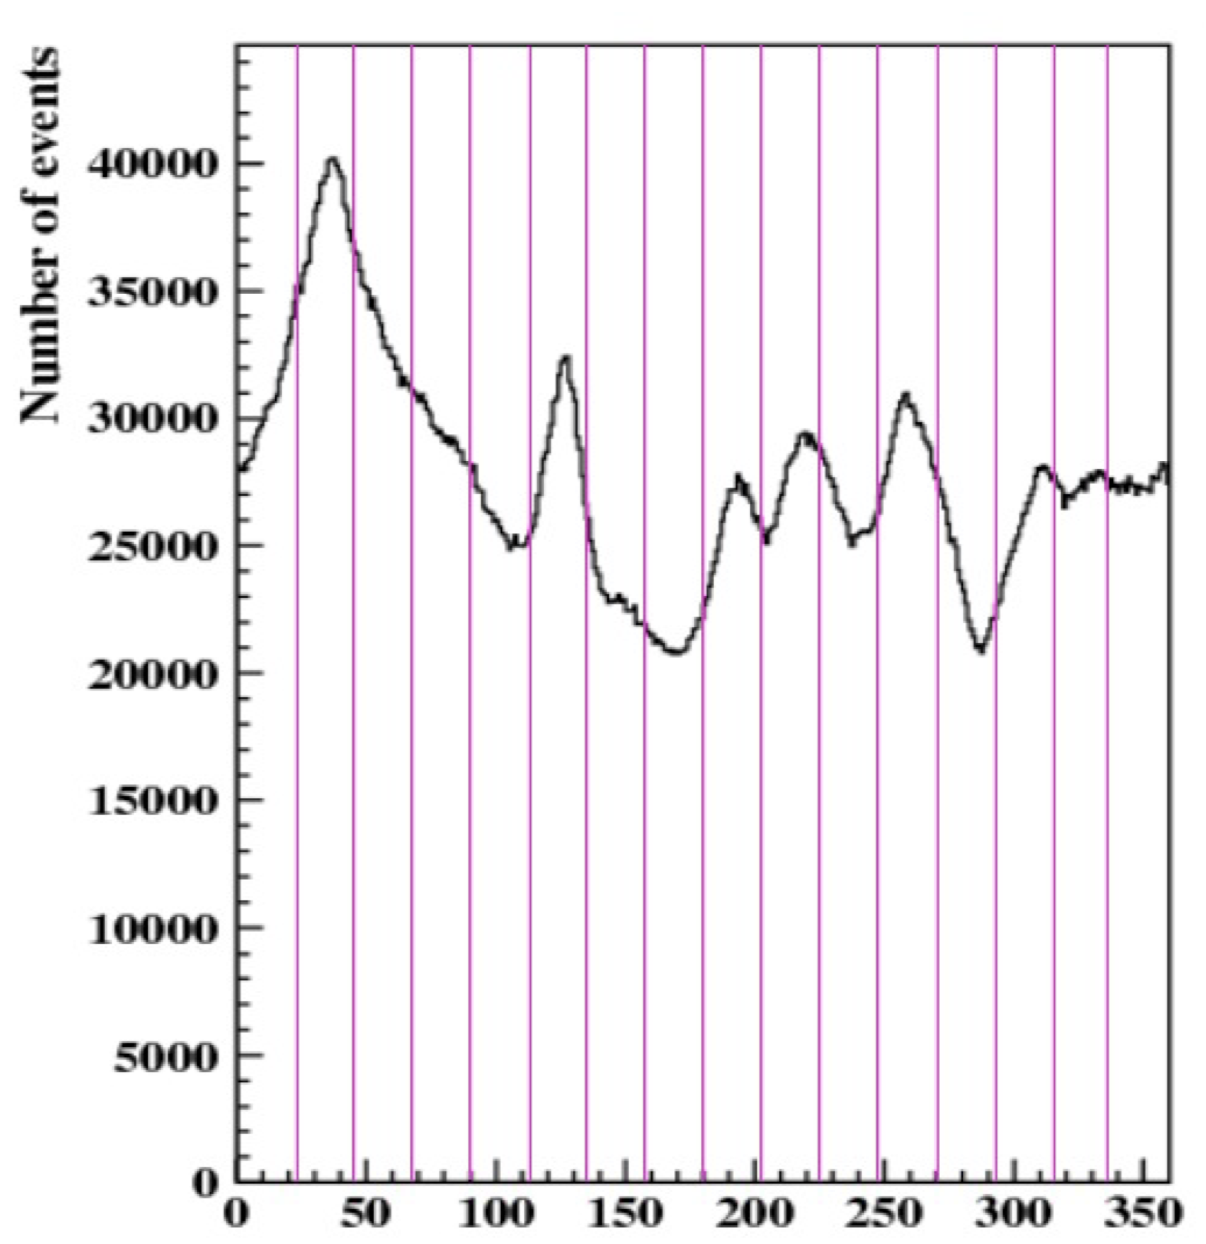
\includegraphics[width=\textwidth]{phi-map}
    \caption{The distribution of azimuthal angles of muons at the DUNE far detector site at SURF.}
    \label{fig:SurfProf_Azi}
  \end{subfigure}
  \caption[The correlation between the surface profile and distribution of azimuthal angles at the DUNE far detector site]
          {The correlation between the surface profile and distribution of azimuthal angles at the DUNE far detector site. The quadrants have been divided into four angles of equal size. The azimuthal angle, calculated as the angle from East (pointing to the right in Fig.~\ref{fig:SurfProf_Col}), and increasing counterclockwise, is seen to follow the contours of the surface profile.}
\end{figure}

Given these parameters, the muon flux when assuming a spherical detector geometry, without simulating a detector cavern, is given by Table~\ref{tab:MUSUNflux}. \\
\begin{table}[h!]
\caption[Muon flux parameters as calculated with MUSIC/MUSUN.]
        {Muon flux parameters as calculated with MUSIC/MUSUN.}
\centering
\label{tab:MUSUNflux}
\begin{tabular}{c c c c}
\toprule
{Total flux (cm$^{-2}$ s$^{-1}$)} & {Mean E$_{\mu}$ (GeV)} & {Mean slant depth (m w.e)} & {Mean $\theta$ ($^{\circ}$)} \\ 
\midrule
5.66 $\times$ 10$^{-9}$           & 283                    & 4532                       & 26                           \\
\bottomrule
\end{tabular}
\end{table}

The muons simulated for DUNE are sampled on the surface of a box surrounding the detector hall, that also encompassed 7 m of rock above the cavern, and 5 m of rock on all other sides. This is to ensure that there is sufficient rock to induce cascades both above and around the detector hall, as it is mainly the secondaries produced in these interactions, which then enter the detector, that are of concern to nucleon decay searches. This will be discussed in Section~\ref{sec:DUNENDK}. The size of the box the muons are sampled from is 74.43 $\times$ 29.54 $\times$ 30.18 m$^3$, compared to the simulated cryostat which has dimensions, 61.62 $\times$ 14.94 $\times$ 13.58 m$^3$. The dimensions are given as length $\times$ width $\times$ height. The muons are sampled randomly according to their energy spectrum, for a given zenith and azimuthal angle, using the angular distribution obtained with MUSIC. \\

Before this could be done however, MUSUN had to be incorporated into the DUNE software framework, as it has previously been maintained in FORTRAN as an external package. This involved building on the work done by the LZ collaboration in porting the code to C++~!!!!!citep{Kareem}. The process by which this was done was to first reproduce the distributions produced by the LZ collaboration using the DUNE software framework. Once the distributions could be reproduced for the Davis shaft at SURF, the muon distributions produced by the original FORTRAN code for the DUNE detector location were reproduced. The distributions produced by the DUNE software framework are shown in Figure~\ref{fig:MUSUNIncorp}, these are seen to be consistent with the same distributions shown in~\citep{MUSUNLBNE}. The initial positions of 10,000 muons generated in LArSoft around the simulated DUNE 10 kt module are shown in Figure~\ref{fig:10ktPos}. The initial positions of the muons are shown as blue points, whilst the cryostat is a single black box and each TPC is a single red box. \\

\begin{figure}[h!]
  \centering
  \begin{subfigure}{0.45\textwidth}
    \centering
    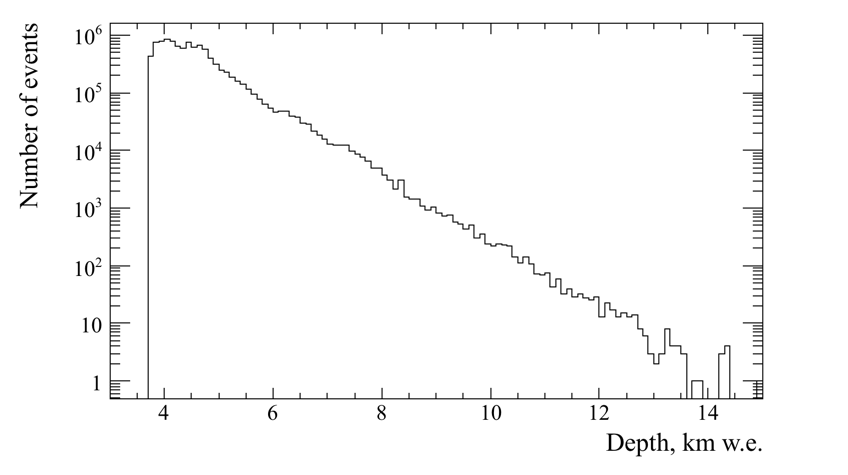
\includegraphics[width=\textwidth]{DepthCan}
    \caption{Distribution of slant depths.}
  \end{subfigure}
  \hspace{0.08\textwidth}
  \begin{subfigure}{0.45\textwidth}
    \centering
    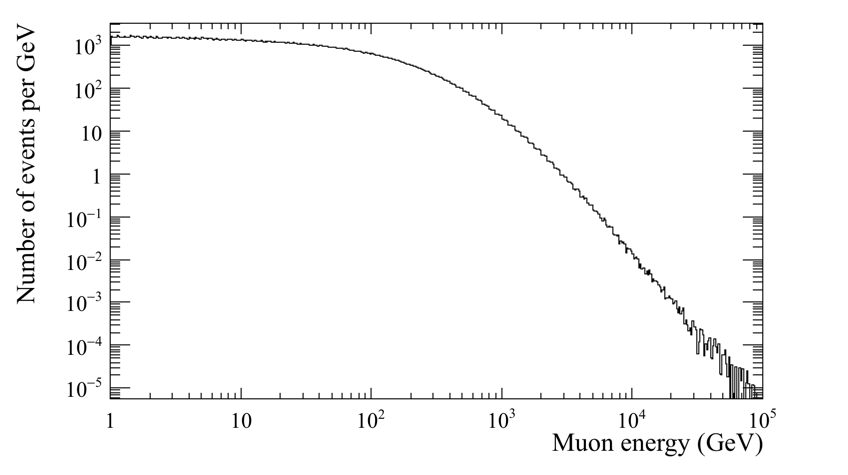
\includegraphics[width=\textwidth]{EnergyPerGeVCan}
    \caption{The energy spectrum of muon energies.}
  \end{subfigure}
  % ========
  \begin{subfigure}{0.45\textwidth}
    \centering
    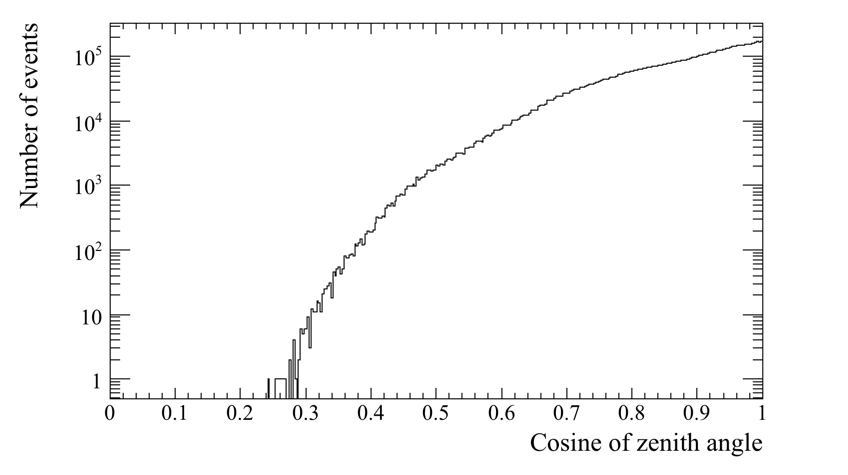
\includegraphics[width=\textwidth]{ZenithCan}
    \caption{Distribution of zenith angles.}
  \end{subfigure}
  \hspace{0.08\textwidth}
  \begin{subfigure}{0.45\textwidth}
    \centering
    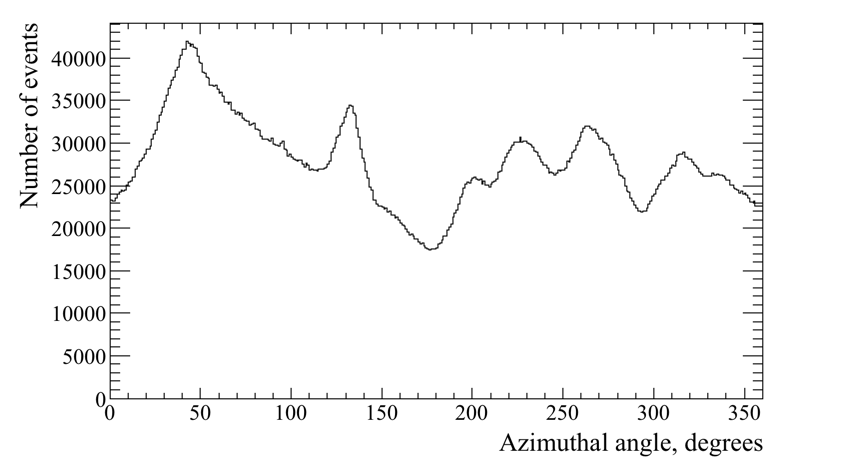
\includegraphics[width=\textwidth]{AzimuthCan}
    \caption{Distribution of azimuthal angles.}
  \end{subfigure}
  % ========
  \begin{subfigure}{0.45\textwidth}
    \centering
    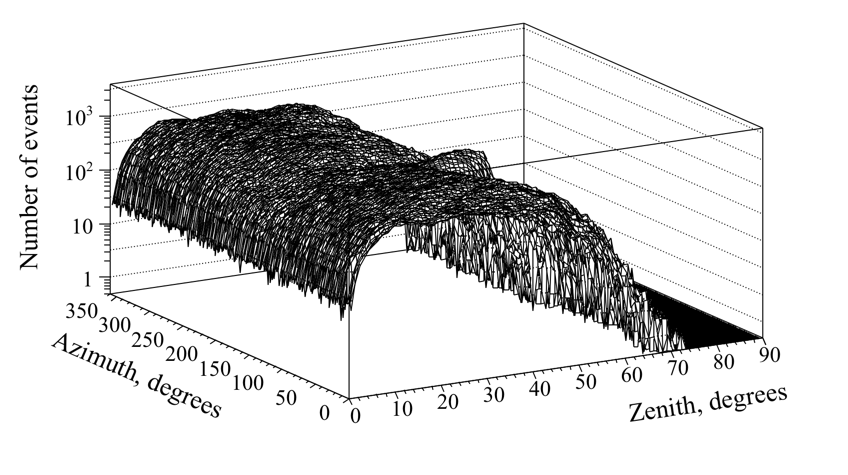
\includegraphics[width=\textwidth]{AziZenCan}
    \caption{The distribution of zenith and azimuthal angles.}
  \end{subfigure}
  \hspace{0.08\textwidth}
  \begin{subfigure}{0.45\textwidth}
    \centering
    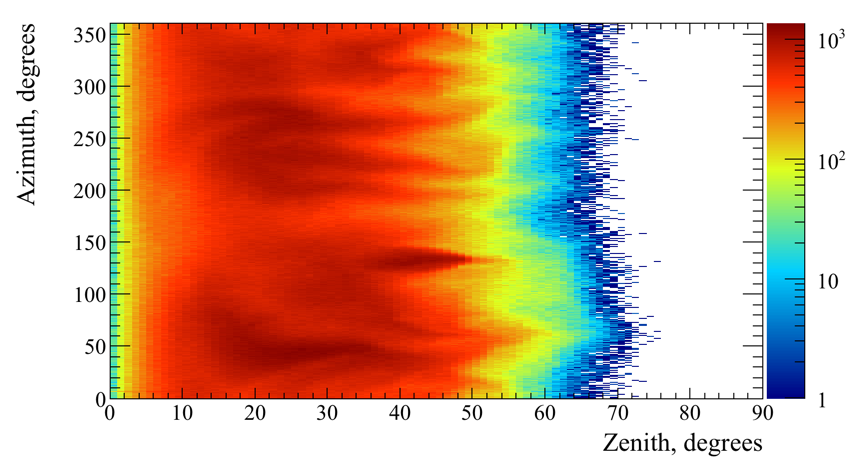
\includegraphics[width=\textwidth]{AziZenColzCan}
    \caption{The distribution of zenith and azimuthal angles, shown with a colour $z$ scale.}
  \end{subfigure}
  \caption[The distributions of some of the important quantities for muons generated by MUSUN in LArSoft]
          {The distributions of some of the important quantities for muons generated by MUSUN in LArSoft. The slant depths and energies of the simulated muons are shown top. The azimuthal and zentih angles of muons are shown middle. Bottom left shows the profile of zenith angle, against azimuthal angle, whilst bottom right shows this with a colour $z$ axis.}
  \label{fig:MUSUNIncorp}
\end{figure}

\begin{figure}[h!]
  \centering
  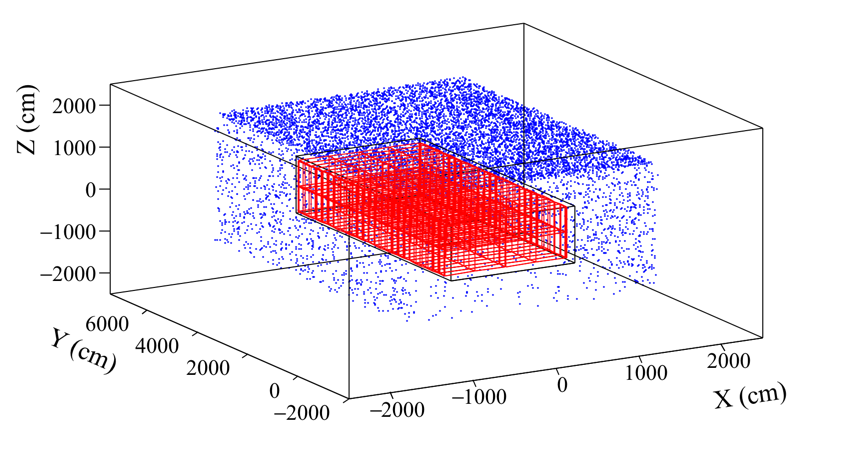
\includegraphics[width=\textwidth]{MuonPosCan}
  \caption[The initial positions of muons generated by MUSUN around a DUNE 10 kt module]
          {The initial positions of muons generated by MUSUN around a DUNE 10 kt module. The initial positions of the muons are shown as blue points, whilst the cryostat is a single black box and each TPC is a single red box.}
  \label{fig:10ktPos}
\end{figure}

It is found that the muon rate through the box upon which the muons are sampled is 0.1579 Hz. This rate is later used to normalise the background event rate in Section~\ref{sec:DUNENDK}. Roughly a third of the muons which are generated pass through the active volume, to give a muon rate through the active volume of 0.053 Hz. \\ 

%********************************** % Fifth Section  *************************************
\section{Nucleon decay channels in DUNE} \label{sec:DUNENDK} %Section - X.5
When searching for rare processes where an experiment is unlikely to see more than a few real signatures, an exhaustive study of the potential backgrounds is required so as to establish that if a signal is observed, it could provide overwhelming evidence for the process. The search for nucleon decay in DUNE is one such process, and so an exhaustive study of the background to nucleon decay is required. As discussed in Section~\ref{sec:BkNDK} cosmogenic muons cause backgrounds to nucleon decay signatures as the secondary particles produced by their interactions are able to mimic the nucleon decay signatures. For this reason it is necessary to simulate this background, and to develop a series of cuts that can be applied to the cosmogenic background to establish that the energy depositions which they cause, are not due to nucleon decays. When doing this, it is important to use a simulation that is as accurate as possible to the DUNE far detector. It is for this reason that MUSUN was incorporated into LArSoft, as the muons which it generates are well matched to the observed muon flux, as described in Section~\ref{sec:FDIncorporation}. \\

To ensure that the background has been properly simulated it is advantageous to simulate many more background events than will be collected by the experiment. As the DUNE detector will run for roughly 20 years, it was decided that an initial sample representing 200 years of detector live time would be simulated. Given that the muon rate through the cavern is 0.1579 Hz, 200 years of detector live time corresponds to roughly 10$^9$ muons. This only represents one of the DUNE 10 kt modules, and so an even larger dataset will be required to represent the full live time of the 4 10 kt modules. For this reason, muons will continue to be generated even though the initial sample size has been reached. \\

Producing samples of this size requires significant computer power, both in terms of running time, and storage space. As such, many of the simulated events are discarded before being saved to disk, through the application of a filter after GEANT4. It is essential that the events which are discarded could not have been mistaken for signal events, and so only very generous cuts are applied. Only events satisfying one of the following cuts are discarded;
\begin{itemize}
\item Contain a muon track of more than 1 m.
\item There are no energy depositions in the entire detector volume.
\end{itemize}
It is envisioned that a muon track of more than a metre would not be misreconstructed. It is also assumed that any signatures observed within one drift window of such a track would not be studied in a nucleon decay search, as there would be doubt as to the authenticity of the signal. Given that the total rate of muons through the active volume is 0.053 Hz, and that the drift time is a few ms, ignoring all times where any track from a cosmogenic muon is present results in less than 0.1\% dead time. The dead time associated with ignoring events with muon tracks of more than 1 m is clearly less than this. This amount of dead time is assumed to be acceptable. \\

After applying this series of cuts, the initial sample of 10$^9$ muons is reduced to XXXX$\times$10$^{XXXX}$ muons which is a much more reasonable sample size to store on tape, and to perform analyses on. It is upon this reduced sample of muons that the cosmogenic background analyses are performed. As discussed in Section~\ref{sec:NDK_Atmos}, the proton decay channel of $p \rightarrow K^{+} + \nu^{e}$ is referred to as the 'Golden Channel' in LAr, this analysis is discussed in~\citep{NDKTFNote}. The related decay of channel of $n \rightarrow K^{+} + e^{-}$ is discussed here. \\

%********************************** % Fifth.First Section  *************************************
\subsection{Cosmogenic background to the $n \rightarrow K^{+} + e^{-}$ decay channel} \label{sec:NDKCosmBk}
As shown in Table~\ref{tab:NDKLim}, the predicted sensitivity that DUNE will have to this channel is much larger than that of Super-K, and so it is an interesting decay mode to study, as DUNE could easily have the best limit for this decay channel. As discussed in Section~\ref{sec:BkNDK}, the cosmogenic background to nucleon decay is predominantly caused by neutral particles such as $K^0$ entering the detector volume, and interacting far away from the detector edges. This is particularly true for the 'Golden Channel,' as shown in Figure~\ref{fig:K0LongBackground}, but it also holds for other channels. This means that it is events such as this which are the main cause for concern when trying to eliminate all cosmogenic backgrounds. \\

As is the case with the 'Golden Channel,' the final state of the decay contains a single charged kaon and so energy constraints can be applied to the kaon that is produced. However, there is also a single electron in the final state, and so this provides further constraints upon the final state. This extra constraint should make it more difficult for a background event to mimic a signal event, as one would expect that the charged kaon and electron would have a common vertex. This is discussed in Section~\ref{sec:NDKSig}. Other constraints that are applied to eliminate background events are; a cut on muon length, a cut on depositions near the detector edges, and criteria about the distribution of deposited energy. The criteria about the distribution of deposited energy is found by considering a sample of simulated decay events, and is discussed in Section~\ref{sec:NDKSig}. These cuts, which are applied sequentially, are outlined below:
\begin{itemize}
\item The event contains energy depositions due to kaons and due to electrons.
\item The event contains at least one kaon track, and at least one electron track.
\item The event contains a single kaon track, and a single electron track.
\item No muon travels more than 20 cm in the detector volume.
\item The event has no energy depositions within 2 cm of the detector edges.
\item The kaon and electron share a common vertex.
\item The energy depositions are within the range which are expected from a nucleon decay event.
\end{itemize}
Inspiration for these cuts can be found in~\citep{Bueno}. The cut on muons was relaxed from a cut on any muon being present to a maximum track length of 20 cm, as this was found to be sufficient. The cuts on the number of pions in the event, were relaxed so as to not expect that all particles are perfectly reconstructed. As the analysis is performed using Monte Carlo truth information, the reconstruction of the kaons and electrons produced are assumed to be perfectly reconstructed though. Similarly, as the energy depositions are not smeared, it is assumed that all deposited charge will be reconstructed, and that the detector characterisation is perfect. This is something which will need to be refined in future analyses, and will be taken into account when the analysis progresses to use reconstructed quantities, as discussed in Section~\ref{sec:NDKImprov}. \\ 

When performing the analysis it is important to be able to trace the particle ancestory. This is so that energy depositions in the detector can be properly assigned, and cuts applied, to the relevant particles. For example, a $\mu^{+}$ is often produced when a $K^{+}$ decays at rest, and this muon may travel more than 20 cm. However, the cut on muon length should not be applied to this muon as it was produced by the decay of the kaon. Similarily, as the kaon interacts in the detector, secondary particles such as pions will be produced. The initial kinetic energy of the kaon can be determined by summing the energy depositions due to these secondary particles, and the energy depositions due directly to the kaon itself. Correctly calculating the initial kaon kinetic energy, through correctly assigning the ancestory of energy depositions, is critical when attempting to verify if an event is a potential signal, as nucelon decay events have very specfic energy criteria. These are outlined in detail in Section~\ref{sec:NDKSig}. \\

For the purposes of this study the definition of a track is that the particle in question has energy depositions which are directly associated with it. This means that it is assumed that an electron will have a short 'track like' segment before it begins to shower. This is an assumption which has been taken from the benchmarking of the shower reconstruction in LArSoft. This definition is used so that it is possible to calculate the positions at which the tracks began and finished depositing energy in the detector. The distance between the kaon initial position, and the electron initial position, is then calculated with respect to these points. These points generally correspond to the Monte Carlo truth start positions, though this is not always the case, as it is possible that they were produced in uninstrumented regions of the detector, such as the gaps between TPCs. The fiducial cut that is applied is only done so with respect to the outer edge of the cryostat, as if it were done with respect to the edge of every TPC in the far detector the loss of volume would be prohibitive. \\

Once the ancestry of energy depositions in the simulation have been correctly accounted for, and the initial kinetic energies calculated, it is possible to observe the distribution of background events as the cuts outlined above are applied. The energy distribution of background events survivng the application of sequential cuts, is shown in Figure~\ref{fig:NDK_CosmoBack_Raw}, and the normalised energy distribution of background events surviving the application of sequential cuts, is shown in Figure~\ref{fig:NDK_CosmoBack_Norm}. The distribution of normalised energies is found by dividing the number of events by the bin energy. \\

\begin{figure}[h!]
  \centering
  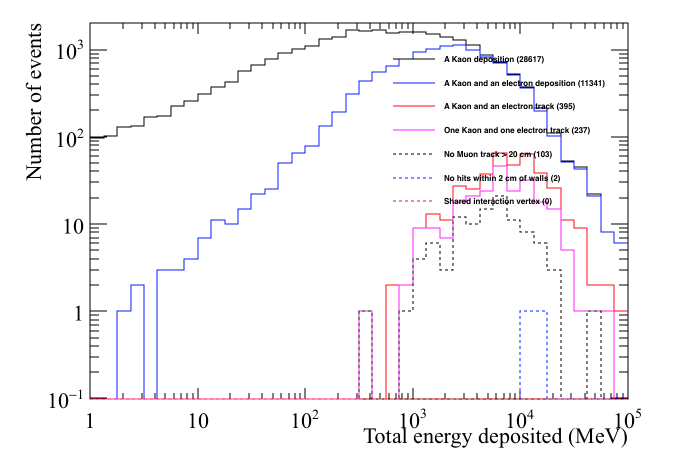
\includegraphics[width=0.8\textwidth]{CosmicBackground_EnergyDepCuts_Raw}
  \caption[The energy distribution of background events surviving the application of sequential cuts in the $n \rightarrow K^{+} + e^{-}$ channel]
          {The energy distribution of background events surviving the application of sequential cuts in the $n \rightarrow K^{+} + e^{-}$ channel. The total energy deposited in the detector is plotted on the $x$ axis.}
  \label{fig:NDK_CosmoBack_Raw}
\end{figure}

\begin{figure}[h!]
  \centering
  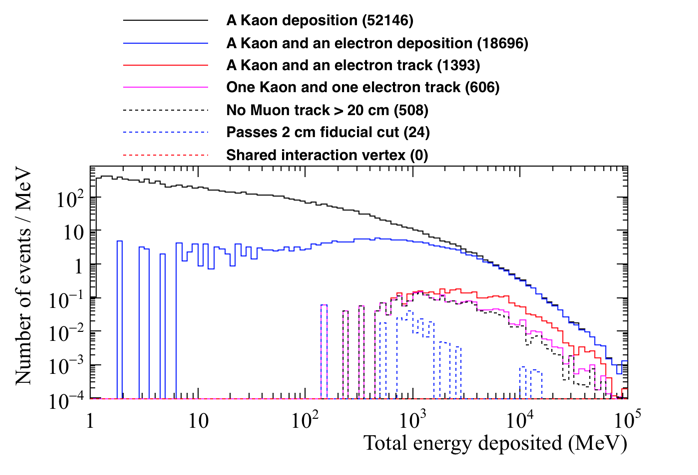
\includegraphics[width=0.8\textwidth]{CosmicBackground_EnergyDepCuts_Norm}
  \caption[The normalised energy distribution of background events surviving the application of sequential cuts in the $n \rightarrow K^{+} + e^{-}$ channel]
          {The normalised energy distribution of background events surviving the application of sequential cuts in the $n \rightarrow K^{+} + e^{-}$ channel. The total energy deposited in the detector is plotted on the $x$ axis. The number of events has been normalised by the bin energy.}
  \label{fig:NDK_CosmoBack_Norm}
\end{figure}

From Figures~\ref{fig:NDK_CosmoBack_Raw} and~\ref{fig:NDK_CosmoBack_Norm}, it can be seen that there are no background events which could mimic a decay signature as there no events which survive the application of all cuts. It is interesting to observe the effect that relaxing some of the cuts has on the number which events which survive previous cuts. 

%********************************** % Fifth.Second Section  *************************************
\subsection{Signal events in the $n \rightarrow K^{+} + e^{-}$ decay channel} \label{sec:NDKSig}

%********************************** % Fifth.Third Section  *************************************
\subsection{Future improvements to nucleon decay studies} \label{sec:NDKImprov}
Thus far the nucleon decay studies have been performed on the Monte Carlo truth information, and so have not used reconstructed objects such as tracks. The extension of the analyses to include work on tracks is an important next step as then the full analysis which would be applied on real data can be tested. Preliminary studies have begun on hit reconstruction, and involve running a filter on the muons used in the earlier analyses. This is because the number of events which are saved to disk would be prohibitive to running the full reconstruction process. As such, only events which meet the following criteria will be reconstructed!!!~citep{ProbsCollabMeetingPres}!!!;
\begin{itemize}
\item A minimum of 10 MeV deposited in the detector volume.
\item A maximum of 3,000 MeV deposited in the detector volume.
\item A maximum of 5 MeV deposited within 10 cm of the detector edge.
\end{itemize}
These criteria are designed to be broad enough that the full range of nucleon decay modes can be studied, including di-nucleon decay modes, hence the maximum deposited energy greatly exceeding the rest mass of a single nucleon. \\
